汽车电子架构变得越发复杂,包括越来越多的传感器、控制器和接口,对通信带宽、链路和速率有了更高的要求。
以太网通信相较于传统的车载通信方式,如 CAN、LIN 等,具有高通信速率的显著优势。


车载以太网协议是一组多个不同层次上的协议簇。从上到下一共分为5层,分别是应用层、传输层、网络层、数据链路层、物理层。5层结构对应于 简化的OSI参考模型,并且提供了各种协议框架下形成的协议簇。
区别于传统以太网,AutoSar对车载以太网的协议架构划分如下:

\begin{figure}[ht]
    \centering
    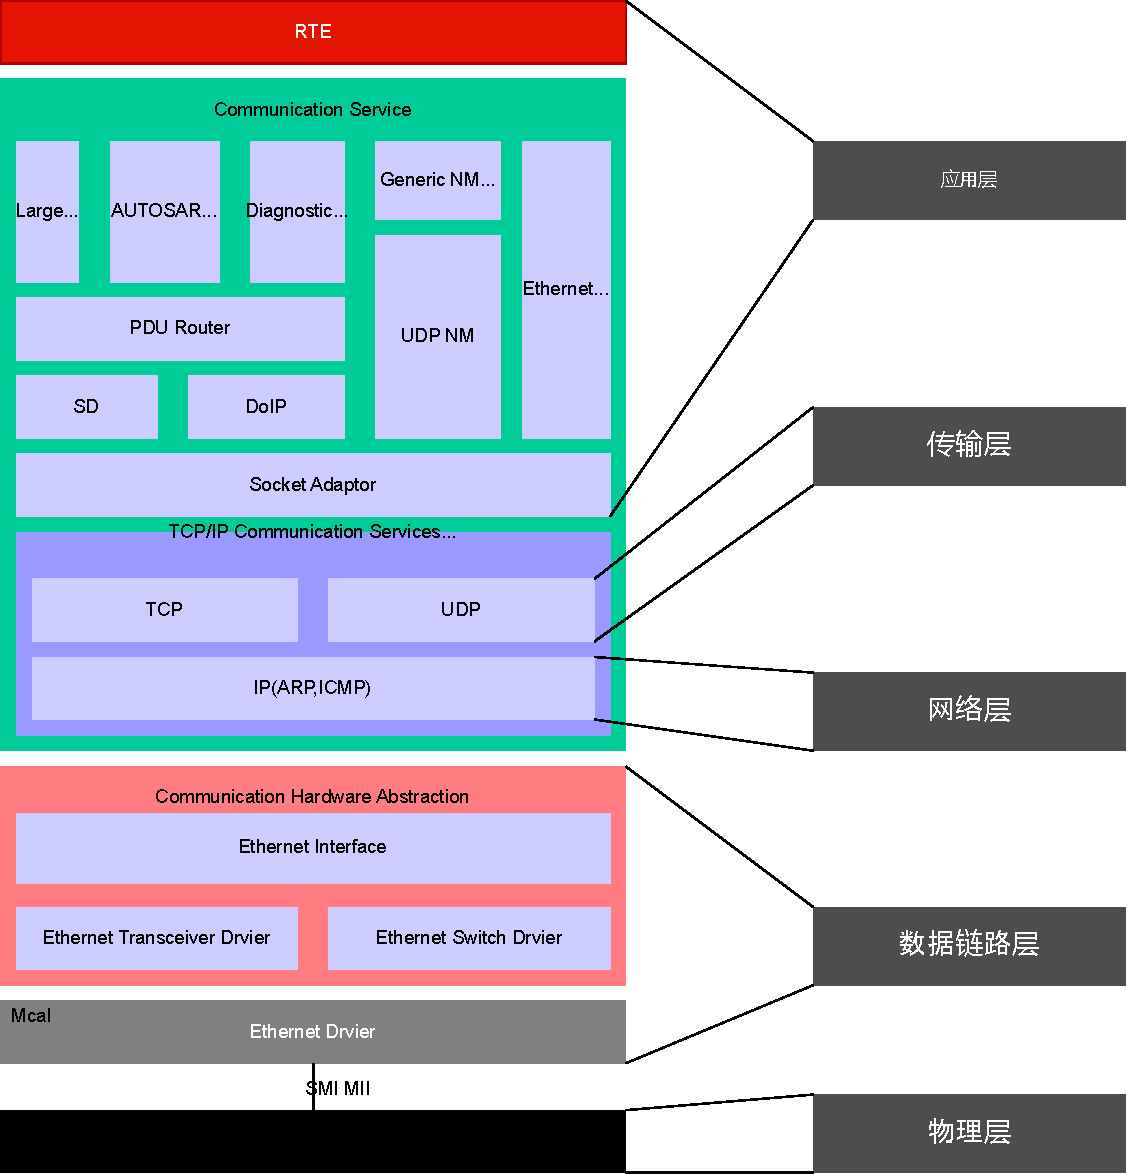
\includegraphics[scale=0.6]{pic/eth_layer.pdf}
    \caption{AutoSar 车载以太网协议架构}
    \label{fig:autosar_eth_layer}
\end{figure}

本章将基于 AutoSar 软件架构及 Vector 工具链完成相关模块的配置,以实现基本的以太网通信。

\section{物理层与链路层}

\subsection{MAC与PHY}

物理层中对以太网硬件的接口形式和编码协议进行了定义。从硬件的角度看,如下图所示,以太网接口电路主要由MAC(Media Access Control)控制器和物理层接口PHY(Physical Layer,PHY)两大部分构成。MAC位于是数据链路层,PHY是物理层;两者通过SMI接口和MII接口连接。

\begin{figure}[ht]
    \centering
    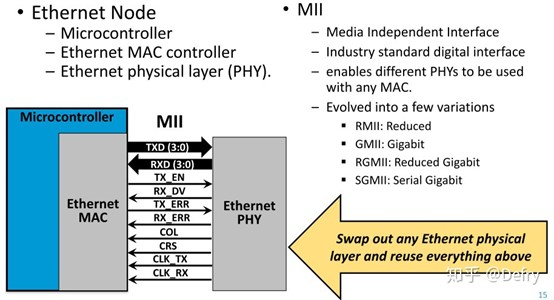
\includegraphics[scale=1]{pic/mii_interface.jpg}
    \caption{MII 接口}
    \label{fig:mii_interface}
\end{figure}

\subsection{SMI 和 MII}
SMI为串行管理接口,以太网MAC通过该接口可以访问PHY的寄存器,通过对这些寄存器操作可对PHY进行控制和管理。SMI接口包括MDIO(控制和管理PHY,以获取PHY的状态)和MDC(为MDIO提供时钟)。MDC由MAC提供,MDIO是一根双向的数据线,用来传送MAC层的控制信息和物理层的状态信息。

MII(Media Independent Interface)即媒体独立接口,MII接口是MAC与PHY连接的标准接口,以太网MAC通过该接口发出数据帧经过PHY后传输到其他网络节点上,同时其他网络节点的数据先经过PHY后再由MAC接收。	

MII接口衍生了很多其他版本,如RMII、GMII、SGMII、RGMII等。这里简要介绍其中的MII和RMII,如下图所示。MII共使用了16根线。其中CRS与COL只在半双工模式有效,而车载以太网固定工作在全双工模式下,故应用在车载以太网需要14根线。

\begin{figure}[ht]
    \centering
    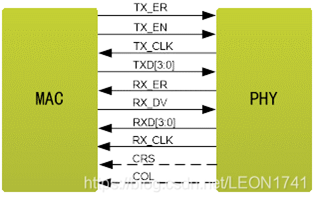
\includegraphics[scale=1]{pic/mii_interface_2.jpg}
    \caption{MII 接口}
    \label{fig:mii_interface2}
\end{figure}

RMII是精简版的MII,数据发送接收均为两根,相比MII减少了4根,另外它整合或减去了一些线,最终RMII只有8根线RMII的接口如下:

\begin{figure}[ht]
    \centering
    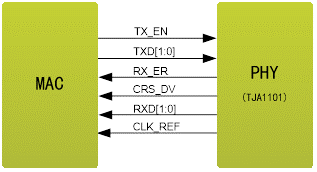
\includegraphics[scale=1]{pic/rmii_interface.jpg}
    \caption{MII 接口}
    \label{fig:rmii_interface}
\end{figure}

\subsection{以太网线束}
对于以太网连接线束,车载以太网与消费用以太网是不同的,首先消费用以太网的标准主要采用10/100BASE-TX和1000BASE-T,其中1000BASE-T是使用RJ45接口,需要四对双绞线共8根线进行数据传输,而10/100BASE-TX则是只使用四对双绞线其中的两对共4根线进行数据传输。

而车载以太网一般都采用带T1的标准,如IEEE 100BASE-T1、IEEE 1000BASE-T1,这些都使用一对双绞线共两根线进行数据传输:

\begin{figure}[ht]
    \centering
    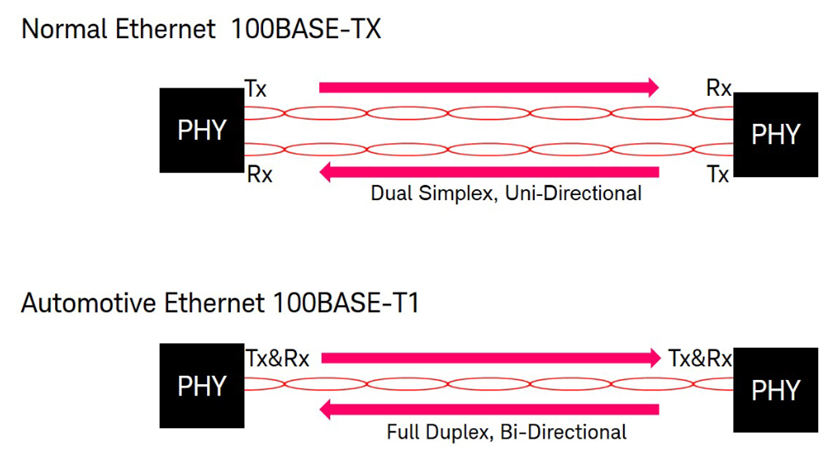
\includegraphics[scale=1]{pic/100basetT1_Tx.png}
    \caption{100BASE-TX 与 1000BASE-T1}
    \label{fig:100basetT1_Tx}
\end{figure}

\subsection{协议转换器}
为了实现100BASE-T1和100BASE-TX协议转换,开发和测试过程中通过协议转换器进行转换,便于在PC上直连测试。如RADMOON转换器。

\begin{figure}[ht]
    \centering
    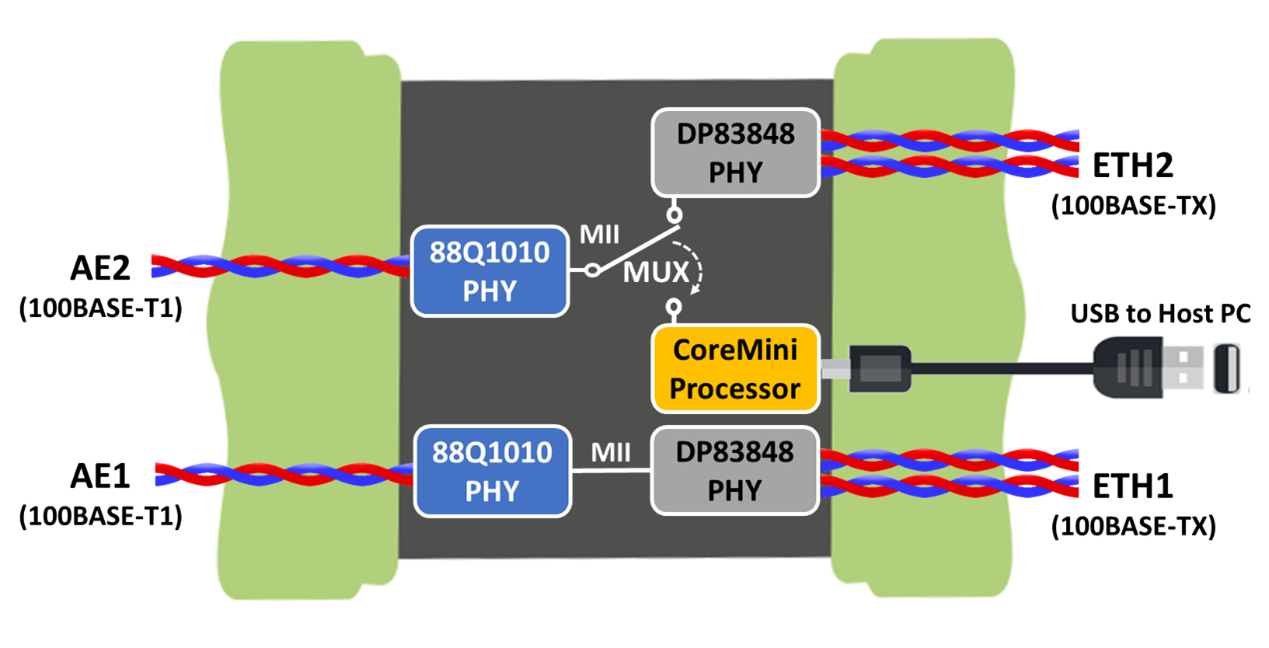
\includegraphics[scale=1]{pic/protocal_convert.png}
    \caption{协议转换器}
    \label{fig:protocal_convert}
\end{figure}

\subsection{交换机}
以太网交换机为车载网络中多个ECU的数据交互提供了桥梁。如下图所示,MCU通过SMI接口控制和管理switch,通过MII接口和switch进行数据交互。

Switch内集成多个PHY,实现多路外部设备的接入。通过多个switch的级联,可以增大节点的接入数量。

\begin{figure}[ht]
    \centering
    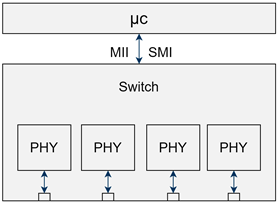
\includegraphics[scale=1]{pic/connect_bt_mcu_switch.png}
    \caption{交换机与MCU连接示意}
    \label{fig:connect_bt_mcu_switch}
\end{figure}

\begin{figure}[ht]
    \centering
    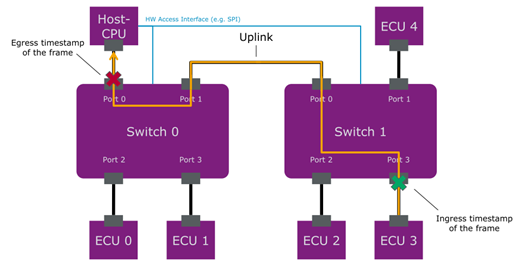
\includegraphics[scale=1]{pic/switch_cap.png}
    \caption{Switch级联}
    \label{fig:switch_cap}
\end{figure}

Switch 主要支持以下功能:
\begin{itemize}
    \item 端口设备MAC地址的自学习,ARL表管理。
    \item 端口VLAN管理
    \item 端口镜像功能
    \item 端口状态信息及故障信息处理 
\end{itemize}

\subsection{以太网帧}
对于上层交付的PDU,通过添加帧头和帧尾使之成为帧,最终在数据链路上传输。这样封装好的帧称为以太网帧,以太帧有多种类型,不同类型的帧具有不同的格式和MTU值,但在同种物理媒体上都可同时存在。目前常用的为Ethernet II帧格式。如下图所示:

\begin{figure}[ht]
    \centering
    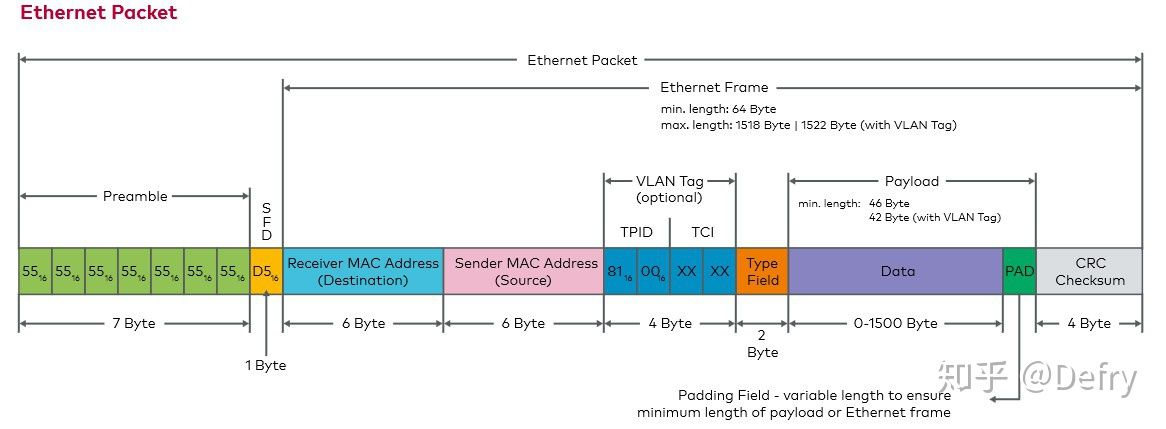
\includegraphics[scale=0.6]{pic/eth_mac_format.jpg}
    \caption{Ethernet II帧格式}
    \label{fig:Ethernet_ii_frame}
\end{figure}

其中关键字段说明如下:
\begin{itemize}
    \item 前导码,7字节,通知目标主机准备接受数据。
    \item 帧首定界符,1字节,表示一帧的开始。
    \item MAC地址:6字节*2,项目中由网络工程师根据项目需求给各个控制器分配私有MAC地址(包括车内单播和组播地址)。
    \item Vlan标签,4字节。
    \item 帧类型:常用以太网帧类型如0x0800(IPv4), 0x0806(ARP),0x8100(VLAN Tag)
    \item 帧校验序列,4字节CRC校验值
\end{itemize}

\begin{figure}[ht]
    \centering
    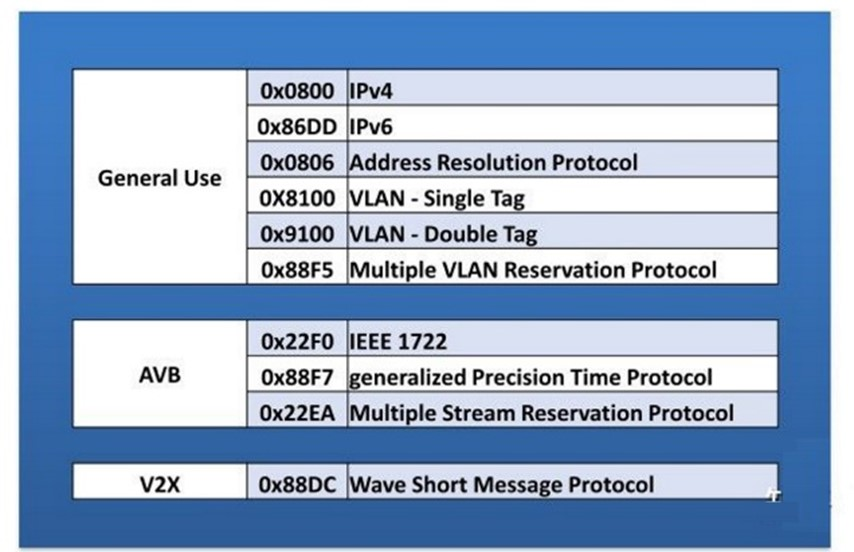
\includegraphics[scale=1]{pic/Ethernet_frame_type.jpg}
    \caption{常用以太网帧类型}
    \label{fig:Ethernet_frame_type}
\end{figure}

\subsection{VLAN}
VLAN主要目的是将一个LAN在逻辑上划分成多个广播域。相同VLAN内的控制器间可以直接通信,而不同VLAN间不能直接通信,从而将广播报文限制在一个VLAN内。当设备数目较多时可以有效隔离广播报文和提升网络质量。

车内网络中为不同节点或诊断设备分配了一个或多个VLAN ID。对于网关节点,为实现车内网络中各以太网节点间的通信需要两步,一是网关自身具有对需求要求的VLAN标签的以太网报文进行处理的能力;二是,配置switch各个端口的VLAN处理功能,实现各节点间基于VLAN的通信。

\subsection{链路聚合}
链路聚合\cite{Link_Aggregation}(英语:Link Aggregation)是一个计算机网络术语,指将多个物理端口汇聚在一起,形成一个逻辑端口,
以实现出/入流量吞吐量在各成员端口的负荷分担,交换机根据用户配置的端口负荷分担策略决定网络封包从哪个成员端口发送到对端的交换机。
当交换机检测到其中一个成员端口的链路发生故障时,就停止在此端口上发送封包,并根据负荷分担策略在剩下的链路中重新计算报文的发送端口,
故障端口恢复后再次担任收发端口。链路聚合在增加链路带宽、实现链路传输弹性和工程冗余等方面是一项很重要的技术。

\subsubsection{链路聚合原理}

\begin{itemize}
    \item 把聚合后得到的逻辑链路称为聚合链路,把聚合链路中的每一条物理链路称为成员链路。
    \item 把聚合后得到的逻辑端口称为聚合端口,把聚合端口中的每一个物理端口称为成员端口。
    \item 聚合链路也被称为Eth-Trunk链路,聚合端口也被称为Eth-Trunk端口。
\end{itemize}

\begin{figure}[ht]
    \centering
    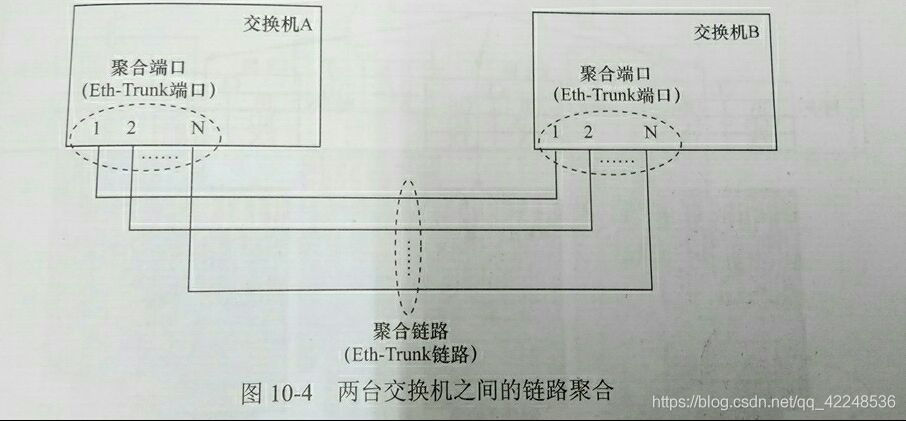
\includegraphics[scale=0.5]{pic/20190414170741211.jpg}
    \caption{交换机链路聚合}
    \label{fig:switch_link_aggre}
\end{figure}

交换机A是怎样通过自己的 Eth-Trunk 端口向交换机 B 的 Eth-Trunk 端口发送帧的?

\begin{enumerate}
    \item 来自交换机A的其他端口的帧进入到Eth-Trunk端口的帧发送队列;
    \item Eth-Trunk端口的帧分发器(FD)将这些帧按照某种算法依次发给成员端口。FD的分发顺序是:先将Frame A发给某个成员端口,再将Frame b发给某个成员端口,依次类推;
    \item 每个成员端口按照常规方法将来自FD的帧发送到自己的物理链路上。如图\ref{fig:switch_link_aggre_transmit}所示。
\end{enumerate}

假若FD能够非常均匀的将帧分发给不同的成员端口,则 Eth-Trunk 端口的带宽就等于各成员端口的带宽之和,而 Eth-Trunk 链路的带宽就等于各成员链路的带宽之和。

但是,FD 对帧的分发并不是非常均匀的,所以 \textcolor{red}{\textbf{Eth-Trunk 链路实际上能够提供的最大的链路带宽一般会小于各成员链路带宽的总和}}。

\begin{figure}[ht]
    \centering
    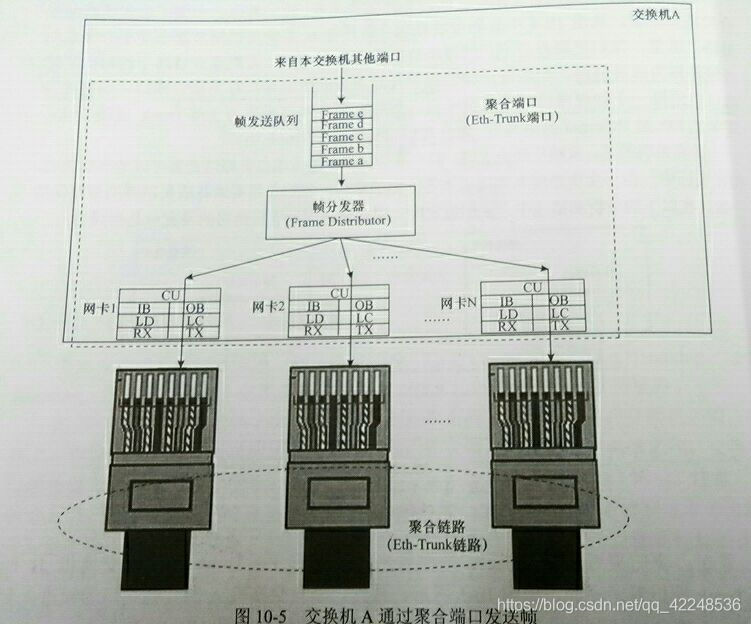
\includegraphics[scale=0.5]{pic/20190414171718383.jpg}
    \caption{链路聚合数据发送}
    \label{fig:switch_link_aggre_transmit}
\end{figure}

交换机B是怎样从自己的Eth-Trunk端口接收到来自交换机A的Eth-Trunk端口发送过来的帧?

\begin{enumerate}
    \item 每个成员端口会按照常规方式接收来自物理链路上的帧,将接收到的帧送到Eth-Trunk端口的帧收集器(FC);
    \item 当帧“完全进入”(指:帧的末尾也进入到FC中)到FC中后,FC会将它送至Eth-Trunk端口的帧接收队列中;
    \item 最先完全进入FC的帧是Frame a,其次是Frame b,等等类推。
    \item Eth-Trunk端口的帧接收队列中的帧会被依次的送往交换机B 的其他端口。
\end{enumerate}

\begin{remark}
    链路聚合的基本原理就是“流量分担”原理:多条成员链路共同分担了聚合链路的总流量。如果聚合链路中的某一条成员链路发生故障而中断了,那么聚合链路的总流量会继续呗其他的成员链路来分担(本该由故障链路所分担的流量将会被FD转移到其他的成员链路)。
\end{remark}

\subsubsection{链路聚合乱序问题}
所谓的乱序现象就是指:交换机B的帧接收队列中帧的排序不同于其在交换机A的帧发送队列中的顺序。乱序现象分为两种:有害乱序、无害乱序。
有害的乱序:会多少的对网络应用程序有所影响。无害的乱序:交换机B的帧接收队列中发生的乱序现象是一种无害的乱序。

聚合链路在工作的过程中,由于帧的长度有所不同,则帧的传输时间就会有所不同,有长有短的时间,同时不同的帧所经过的成员链路也可能不同,
所有在一般情况下总是会出现乱序现象。虽然无法避免乱序现象的发生,但是可以尽可能的避免有害乱序现象的发生。

避免有害乱序现象的关键是:\textbf{聚合端口的FD是怎样将帧分发给不同的成员端口的}。

\subsubsection{Conversation 概念}
一个Conversation是指由若干个帧组成的一个集合,该集合中的不同的帧在接收端的聚合端口的帧的接收队列中的先后顺序必须与它们在发送端的聚合端口的帧的发送队列中的先后顺序保持一致。如果保持了一致,则一定不会发生有害乱序现象;若没有保持一致,则一定会发生有害乱序现象。

\begin{remark}
    不同的Conversation之间的交集必须是一个空集,即同一个帧,不能既属于这个Conversation,又属于另外一个Conversation;一个帧不能不属于任何Conversation。
\end{remark}


聚合端口需要遵从的分发原则:
\begin{enumerate}
    \item 同一个Conversation中的帧,必须被分发给同一条成员端口(可避免有害乱序现象);
    \item 不同Conversation中的帧,可以被分发给同一个成员链路,也可以被分发给不同的成员链路(可实现流量分担);
\end{enumerate}

图\ref{fig:switch_link_aggre_conversation_transmit}中:交换机A的聚合端口首先会对帧的发送队列中的帧进行Conversation划分,
划分的方法是:把具有相同目的MAC地址的帧分进同一个Conversation,而且要保证同一个Conversation中的帧都具有相同的目的MAC地址。
\begin{figure}[ht]
    \centering
    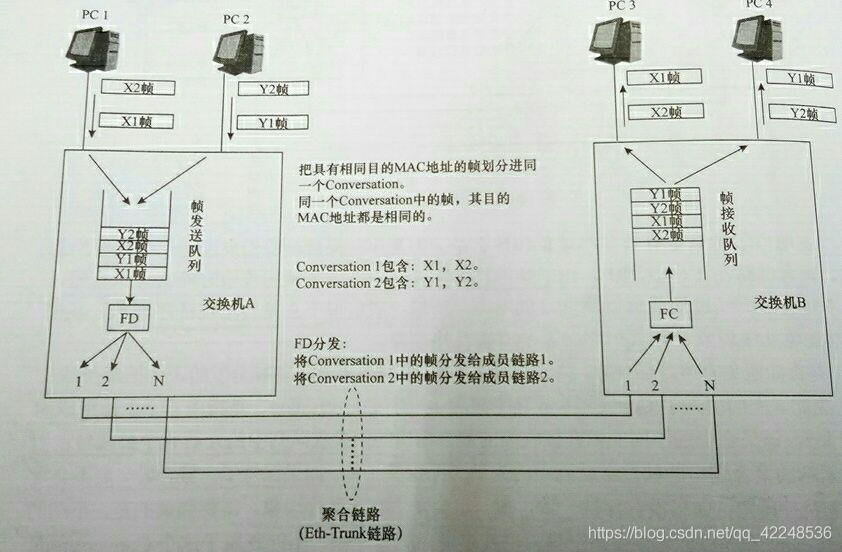
\includegraphics[scale=0.5]{pic/20190414180436629.jpg}
    \caption{链路聚合数据Conversation发送}
    \label{fig:switch_link_aggre_conversation_transmit}
\end{figure}

在实际的链路聚合实现中,聚合链路的FD需要根据HASA算法来定义出恰当的Conversation,然后再对不同的Conversation进行分发。(该图中的目的MAC地址被选择成用来定义Conversation的参考量)。

在实际的网络环境中,聚合链路的两端的设备属性(如:交换机和路由器,等等)以及上层应用的属性,都需要称为确定Conversation的参考量的考虑因素,最终可能参考的是目的MAC地址或者源MAC地址,等等。

\subsection{ENET 中断分析}

ENET 由中断触发到上层数据接收并处理的过程见下图。

\begin{figure}[ht]
    \centering
    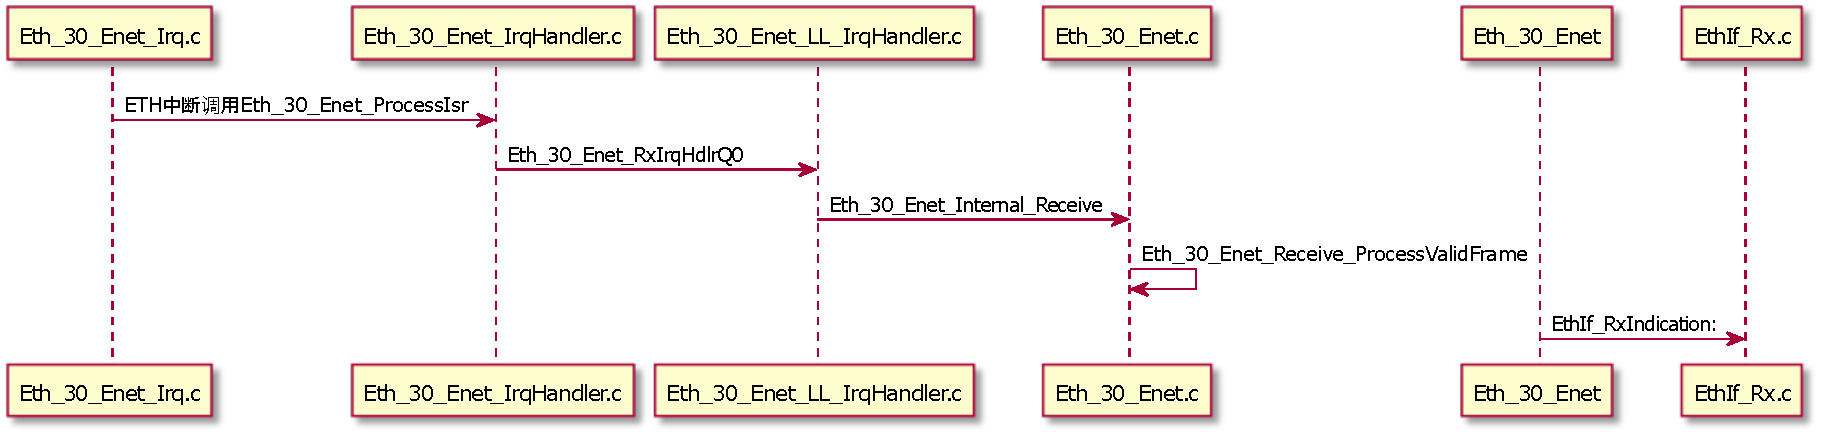
\includegraphics[scale=0.5]{pic/eth_isr.pdf}
    \caption{ENET 中断代码调用}
    \label{fig:enet_isr}
\end{figure}

其中 \lstinline{Eth_30_Enet_Irq.c} 中包含 \lstinline{OS} 中配置的 \lstinline{ENET} 中断处理函数:

\begin{lstlisting}[language=C]
ISR( EthIsr_EthernetCnt_MCU_Ctrl_ad7672f0_EthInterruptServiceRoutine_Q0Rx );
ISR( EthIsr_EthernetCnt_MCU_Ctrl_ad7672f0_EthInterruptServiceRoutine_Q0Tx );
\end{lstlisting}

后续通过 \lstinline{Eth_30_Enet_Internal_Receive} 处理接收到的数据帧,其中由 \lstinline{Eth_30_Enet_Receive_ProcessValidFrame} 验证数据帧后,由 \lstinline{EthIf_RxIndication} 传至上层模块。

